
\section{Elementos Visuais}
Os personagens foram baseados em estatuetas artesanais conforme anexos que acompanham suas descrições. Porém o projeto bebe de variadas fontes de inspiração, e como cada personagem será apresentado em seu ``habitat natural'' planeja-se que ao conhecer os personagens o jogador seja imerso no ambiente em que vive, por esse motivo esta sessão foi separada primeiramente por personagens pois existe uma conexão entre sua fase e o mesmo, e depois por fases em que os três personagens estarão juntos.

\subsection{Duende}
\subsubsection{Ambiente}
O ambiente do Duende, Fulkominn, foi inspirado na Vila de Geiranger, e a partir de imagens dela foi pensado em uma palheta de cores principais para o cenário. Geiranger possui lindas paisagens naturais onde reinam o verde e o azul. Pensando nisso, foi criada uma palheta usando diferentes tons destas cores para realçar a flora e água em abundância nesta fase. Mesmo o personagem possui sua palheta totalmente inspirada nas cores de uma árvore.

\begin{figure}[htb]
	\caption{\label{fig_palhetaFulkominn}Palheta de Cores Fulkominn}
	\begin{center}
	    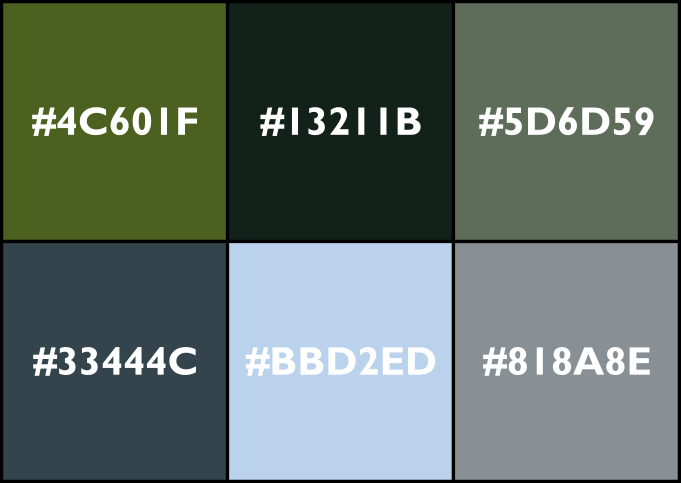
\includegraphics[width=\textwidth/2]{imagens/PaletaGeiranger.png}
	\end{center}
	\legend{Fonte: Autoria Nossa}
\end{figure}

\subsection{Personagem}

\begin{figure}[htb]
	\caption{\label{duendeRef}Estatueta de Duende}
	\begin{center}
	    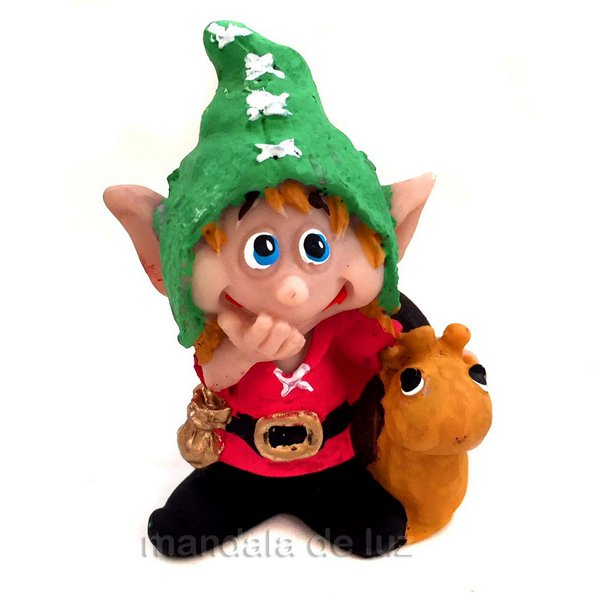
\includegraphics[width=\textwidth/2]{imagens/duendeRef.jpg}
	\end{center}
	\legend{Fonte: Mandala de Luz, 2012}
\end{figure}



\begin{figure}[htb]
	\caption{\label{duendePos}Arte Conceitual Duende}
	\begin{center}
	    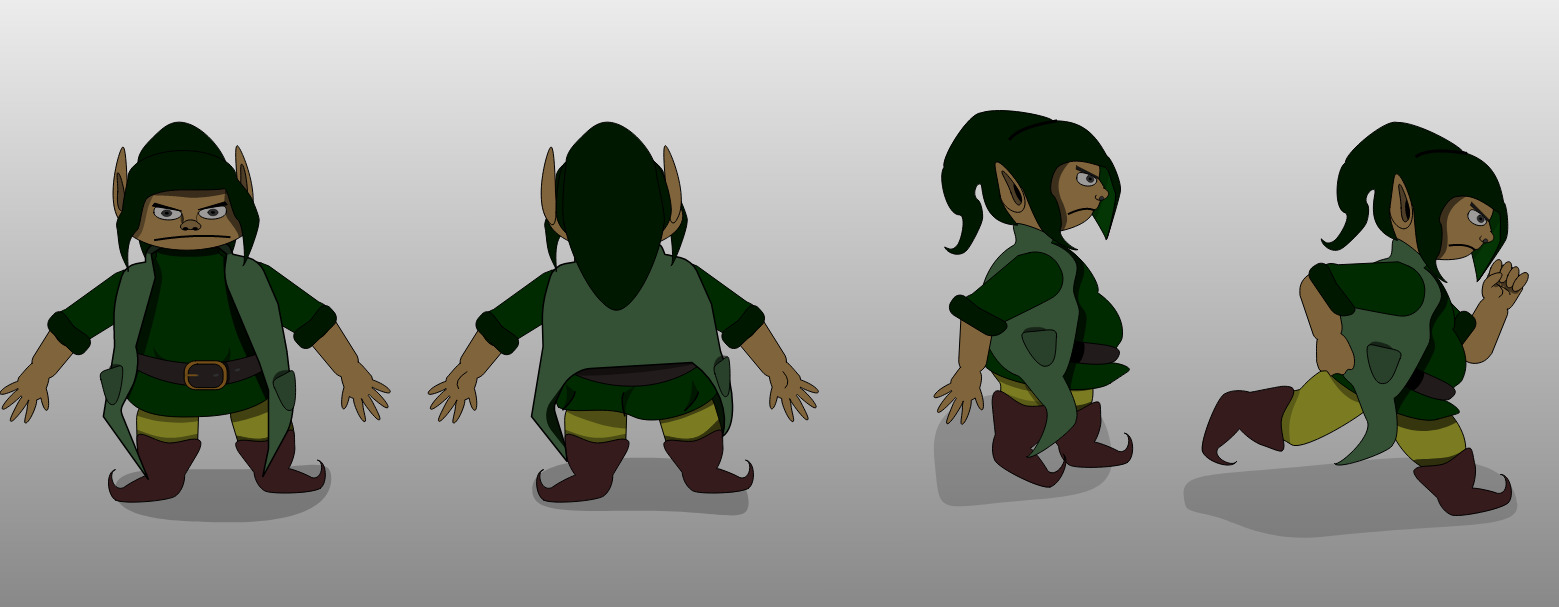
\includegraphics[width=\textwidth]{imagens/duendePosicoes.jpeg}
	\end{center}
	\legend{Fonte: Autoria Nossa}
\end{figure}

\clearpage

\subsection{Xamã}

\subsubsection{Ambiente}
O ambiente do Xamã foi inspirado no parque nacional de Mesa Verde nos Estados Unidos, que é um sítio arqueológico com construções Pueblo. Esta antiga civilização se instalava no interior de grandes cânions, criando suas casas com barro e pedras. O ambiente tem presença massiva de marrom cor de barro com uma tímida contribuição de verde, sem variações de tons. Por essa razão, a palheta foi definida nestas duas cores, com uma aposta em mais de um tom para evitar a monotonia na fase.

\begin{figure}[htb]
	\caption{\label{fig_paletaMesa}Paleta de Cores Ambiente Xamã}
	\begin{center}
	    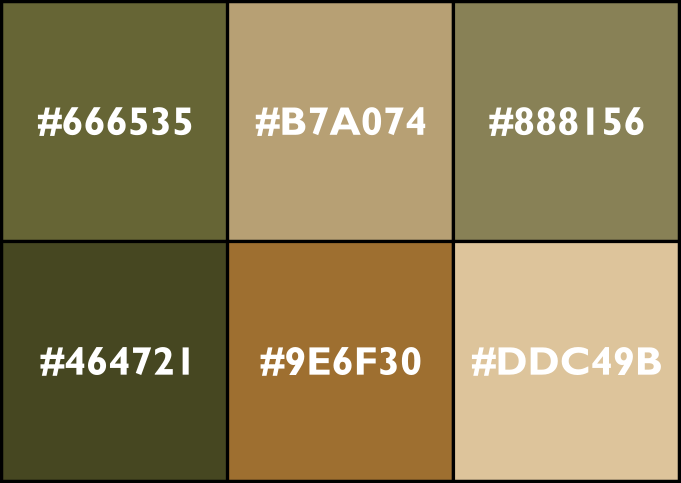
\includegraphics[width=\textwidth/2]{imagens/PaletaMesaVerde.png}
	\end{center}
	\legend{Fonte: Autoria Nossa}
\end{figure}

\subsubsection{Personagem}
Como existem poucos registros dos povos Pueblo, ou Anasazi, optou-se por utilizar referências dos povos Hopi, Ute, Zuni e Navajo para a construção física do personagem. Acredita-se que estes povos descendem dos antigos Pueblo. Estas tribos, em especial os Zuni, têm pele marrom avermelhada e utilizam roupas de cores vivas com penas e adornos. Foi definida então uma palheta composta primordialmente por azul, vermelho e branco, imitando as vestes destes povos.

\clearpage

\begin{figure}[htb]
	\caption{\label{fig_conceptXama}Concept Xamã}
	\begin{center}
	    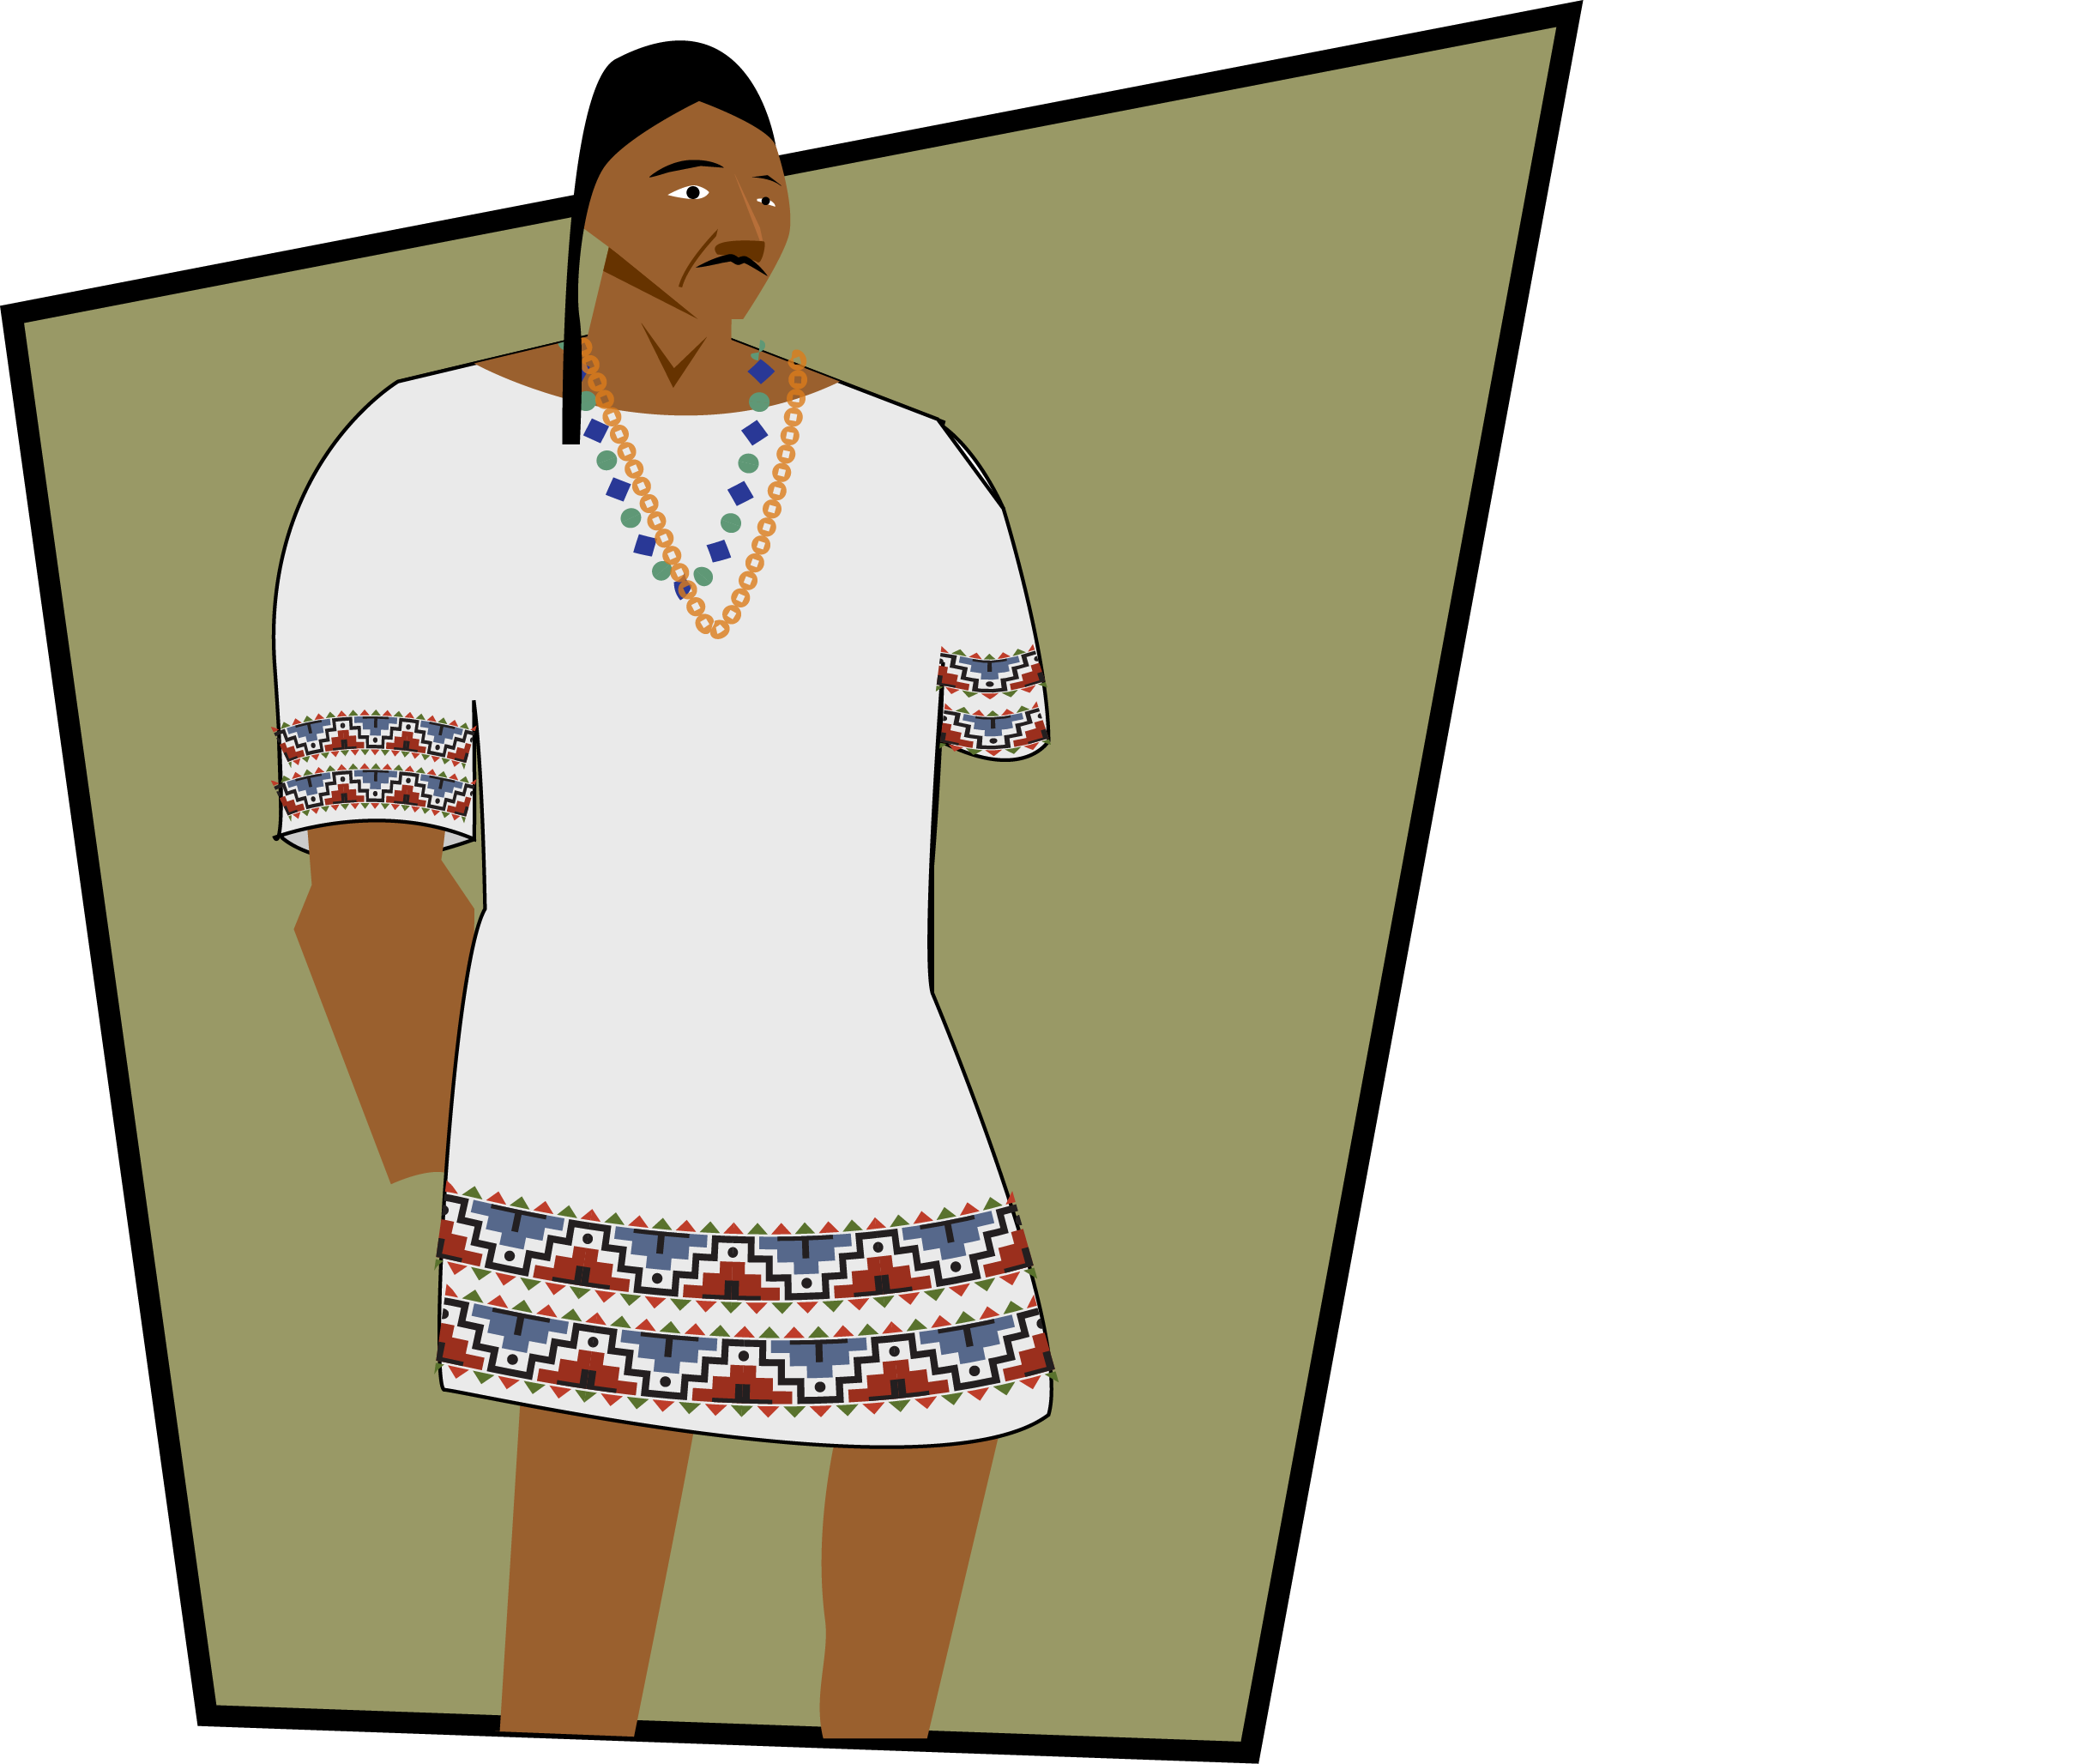
\includegraphics[width=\textwidth/2]{imagens/xama.png}
	\end{center}
	\legend{Fonte: Autoria Nossa}
\end{figure}




\subsection{Bruxa}
\subsubsection{Ambiente}
O ambiente da Bruxa foi inspirado na vila de Killin, no Reino Unido, e a palheta de cores principais pode ser observada na figura \ref{fig_paletaKilin}.

Killin contribuiu muito com noções de arquitetura e flora. Porém, é composta por muito cinza e verde, o que não transmite plenamente o que desejamos. Por esta razão, foi decidido por adicionar mais tons de roxo à palheta, sugerindo misticismo e tons de vermelho, trazendo agitação tanto para a personagem quanto para o cenário. 

\clearpage

\begin{figure}[htb]
	\caption{\label{fig_paletaKilin}Palheta de Cores Ambiente Bruxa}
	\begin{center}
	    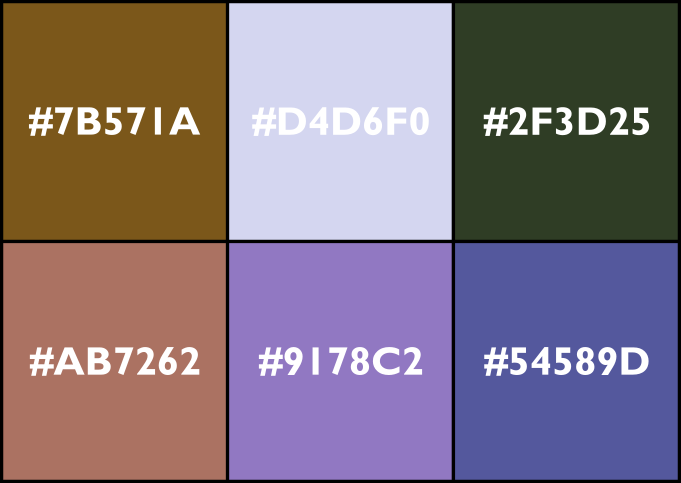
\includegraphics[width=\textwidth/2]{imagens/PaletaKilin.png}
	\end{center}
	\legend{Fonte: Autoria Nossa}
\end{figure}

\subsubsection{Personagem}

\begin{figure}[htb]
	\caption{\label{fig_conceptBruxa}Concept Bruxa}
	\begin{center}
	    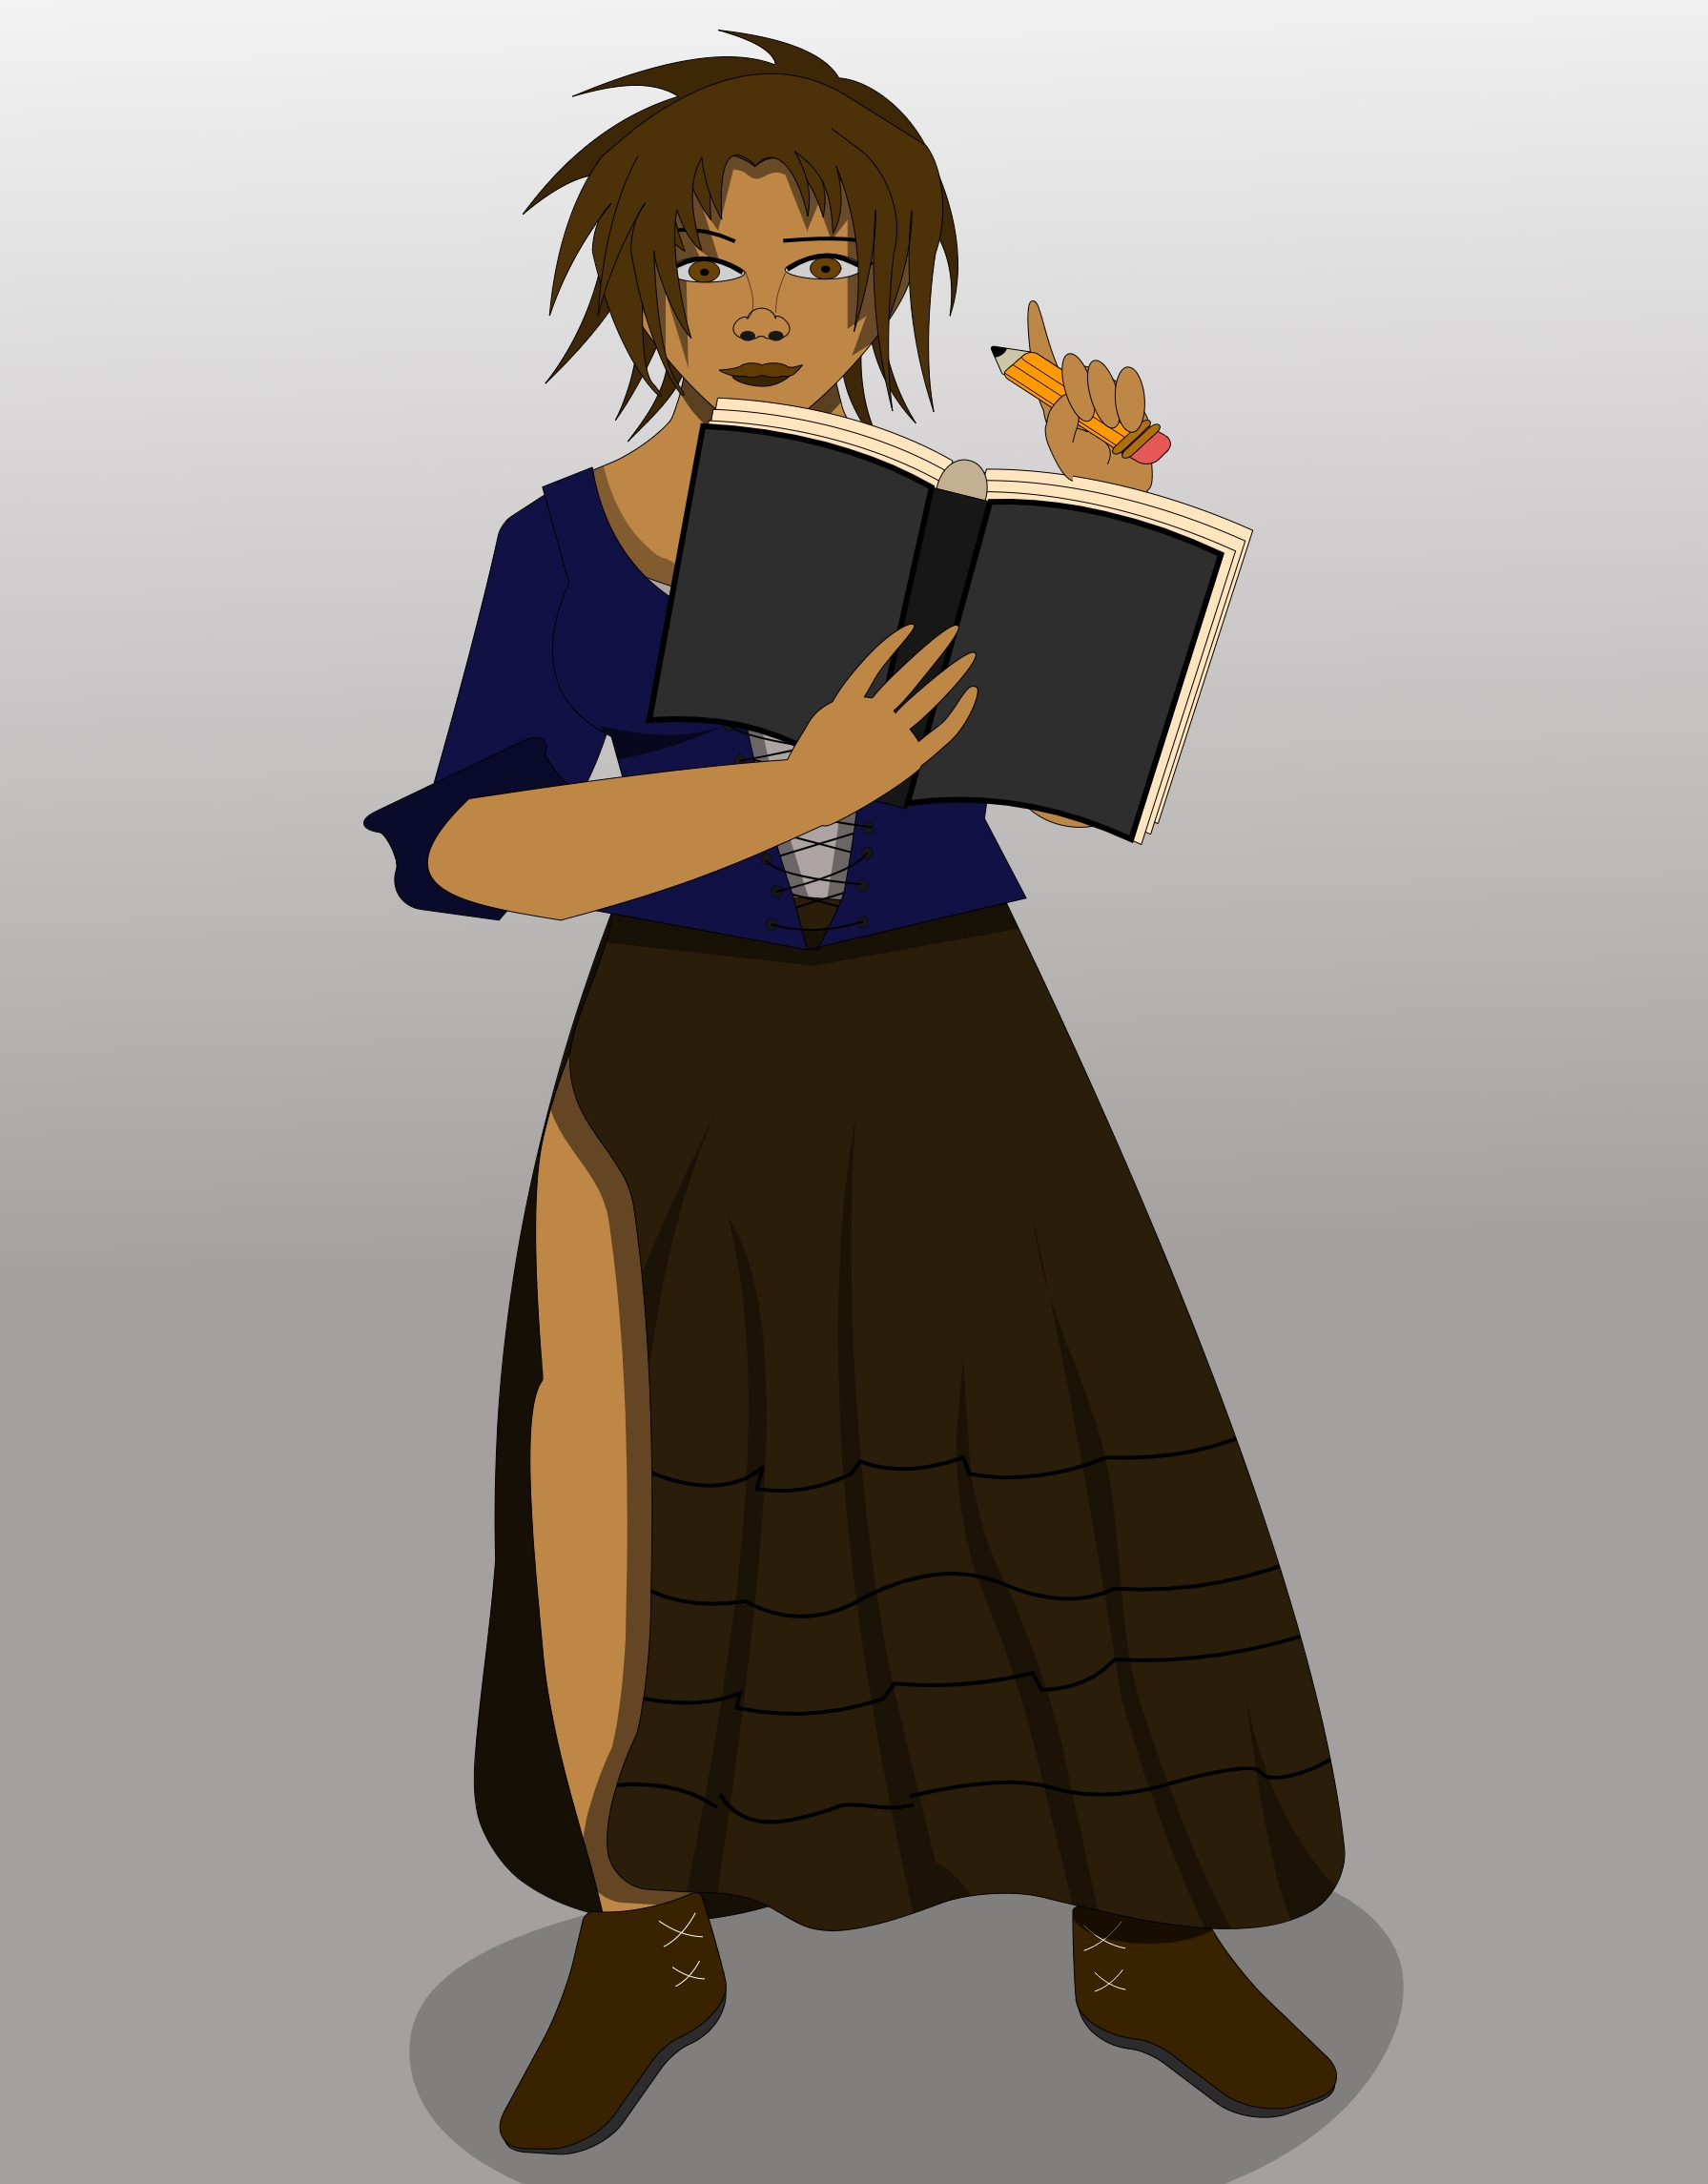
\includegraphics[width=\textwidth/2]{imagens/capaportifolio.jpeg}
	\end{center}
	\legend{Fonte: Autoria Nossa}
\end{figure}


\clearpage

\subsection{Ogof}
O vilão tem em sua palheta muito roxo em tons escuros para remeter misticismo e mistério, mas também um toque de nobreza que impõe respeito. Ogof não possui um ambiente próprio, apenas interage nas fases alheias. Por esse motivo, nota-se uma discrepância nas vestes e palheta de cores deste personagem ao longo do jogo, ajudando a identificá-lo.

\begin{figure}[htb]
	\caption{\label{mago}mago}
	\begin{center}
	    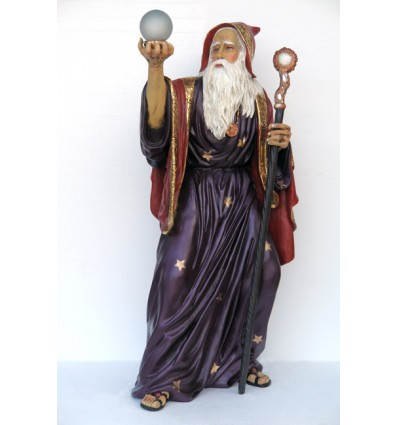
\includegraphics[width=\textwidth/2]{imagens/mago.jpg}
	\end{center}
	\legend{Fonte: Macocaya, 2010}
\end{figure}

\begin{figure}[htb]
	\caption{\label{Ogof}Ogof}
	\begin{center}
	    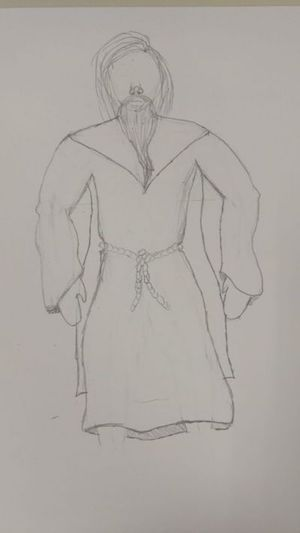
\includegraphics[width=\textwidth/2]{imagens/Ogof.jpg}
	\end{center}
	\legend{Fonte: Autoria Própria - Marina Araujo}
\end{figure}

\clearpage

\subsection{O Templo das Joias}

O Templo das Joias, foi inspirado em no parque Nacional de Tikal na Guatemala, onde estão templos da antiga cultura Maia.

\begin{figure}[htb]
	\caption{\label{fig_paletaTikal}Paleta de Cores Templo das Joias}
	\begin{center}
	    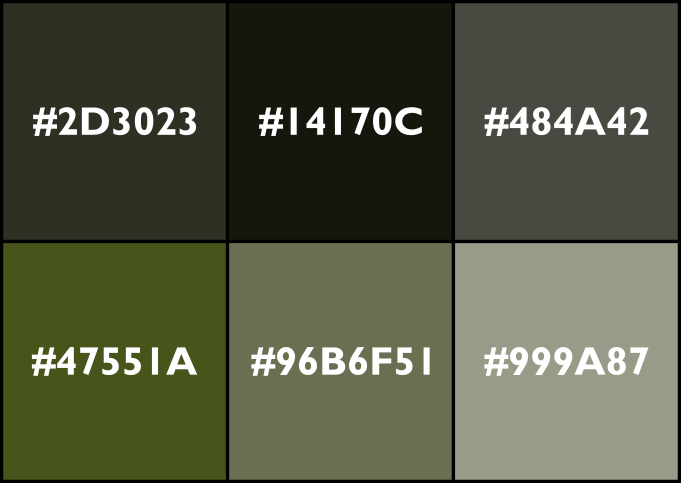
\includegraphics[width=\textwidth/2]{imagens/PaletaTikal.png}
	\end{center}
	\legend{Fonte: Autoria Nossa}
\end{figure}



\section{Elementos Sonoros}

Para uma maior imersão nos ambientes fantásticos que o jogo propoe, as trilha são inspiradas em músicas dos estilos \textit{new age, folk} e músicas tradicionais, nativo americanas, maia, entre outras.

Os elementos sonoros serão produzidos pela equipe, e também serão utilizados efeitos e musicas conseguidas na internet que tenha a licença \textit{Creative Commons}, e serão dados os devidos créditos, tanto no guia impresso do jogo como nas de créditos.
